\documentclass[a4paper]{article}

\usepackage[french]{babel}
\usepackage{geometry}
\usepackage[utf8]{inputenc}
\usepackage{listings}
\usepackage{graphicx}

\usepackage{amsmath}
\usepackage{amssymb}

\date{\today}

\geometry{hmargin=2.2cm,vmargin=3cm}

\title{Rapport de stage}
\author{Emmanuel Rodriguez}



\lstdefinestyle{Python}{%
frame=single,
xleftmargin=2em,
language=python,
numbers=left,
numberstyle=\footnotesize,
columns=[l]flexible,
tabsize=3,
showtabs=true,
tab=$\color{gris!70}\to$,% \rightarrowfill,
backgroundcolor=\color{paille!15},
stringstyle=\color{gris}\
itshape,
showstringspaces=false,
keywordstyle=\color{broudenoix}\bfseries,
commentstyle=\color{vertavocat}\itshape,
% mot des bibliotheques
emph={open,split,readlines,close,append,isdir,groups,Win32_LogicalDisk,argv,match,
VolumeName,showinfo,len},
emphstyle=\color{chocolat}\bfseries,
% import usuels
emph={[2]os,sys,time,re,shutil,wmi,glob,tkMessageBox,path,tkm},
emphstyle={[2]\color{brun}\bfseries\itshape},
}


\begin{document}
\lstset{language=Python} 

\maketitle

\section{Introduction}

On utilise des systèmes aléatoires dans de nombreux domaines de
l'informatique comme les réseaux de communication, systèmes
distribués, systèmes de calculs... Ces systèmes, utilisée pour étudier
et améliorer la performance algorithmique distribuée, sont souvent
composé de nombreux objets en interaction ce qui rend leur analyse
exacte dificile. \\
\smallbreak
Nous nous interesserons dans ce stage a des outils
stochiastiques permetant de montrer que pour de nombreux systèmes, la
performance d'un système composé de N objets a une limite quand N est grand. \\
L'objet de ce stage est s'iteresser a ces systèmes et leur
convergeance. Ainsi qu'a déveloper un simulateur permetant de valider
cette aproximation.

\section{Chaînes de markov à temps continue}
\cite{courscmtc}

\subsection{Définition}

\paragraph{Lois exponentielles}
Une variable aléatoire $T \ $ à valeurs dans $\mathbb{R}_+ \ $ suis la
loi exponentiele de paramètre $\lambda \geq 0$, si  sa fonction de
répartition est donnée par $F(t)=(1-e^{-\lambda t})$ sur
$\mathbb{R}_+$. (et F(t)=0 sur $\mathbb{R}_-^*$).


\subsection{Types de modèles étudiés}
\paragraph{Processus de population markovien a temps continue}
On considère le modèle suivant:

\begin{itemize}
\item N le nombre d'individue répartis dans les diffétents états.
\item un ensemble d'état fini ou dénombrable $S$.
\item un ensemble de transitions avec pour chaque transition une
  fonction de transition associé.
\item $ \{ X_i \}_{i \in S}$une distribution initiale sur l'ensemble des états.
\end{itemize}

On note $X_i$ le nombre d'individues dans l'état $i$.

\paragraph{}
Pour notre etude nous prendrons un modèle de la forme suivante:
\begin{itemize}
\item N la taille de la population
\item un etat initial pour chaque état $X_i$
\item un ensemble de vecteurs $L$ et une fonction $\beta_l : \epsilon
  \rightarrow R^+$ tels que $X^{(N)} \ $ passe de l'état $x$ à
  $x+\frac{l}{N}$ avec un taux $N*\beta_l$.
\end{itemize}

Pour notre étude nous nous limiterons aux modèles ne possedant qu'un
seul point atracteur.

\paragraph{convergence du modèle}
On peur alors montrer $E(X^{(N)})=X_0+\frac{C}{N}+O(\frac{1}{N^2}) \ $
avec $X_0 \ $ le point fixe et $C \ $ un coefficient de correction
dont nous allons chercher la valeur par simulation. 

\subsection{Simulation d'une CMTC}

Pour la simulation, nous partons d'une distribution initiale
donnée.

\paragraph{Methode naive}

Soit $l \in L \ $ un vecteur représentant une transition. Cette
transition est associé au taux $\beta_l \ $. Le système passe d'un
état $X \ $ à $X+\frac{l}{N} \ $ avec le taux $N*\beta_l \ $. Cette
transition aura lieux au temps $expo(N*\beta_l) \ $. Avec expo(i) une
loi exponentielle de paramètre i. On tire donc une loi exponentielle
par transition puis seul la transition qui a lieux en premier est
prise en compte.

Mais il existe  une methode plus rapide et equivalente:

\paragraph{Amélioration}
Pour savoir quelle transition aura lieux en premier on peut plus
simplement choisir une transition $l$ avec proba:
$\frac{\beta_l}{\sum_{i \in L}\beta_i}$, en tirant juste un reel entre 0 et 1 par exemple.
Puis une fois la transition choisi on tire une loi exponentielle de
paramètres $\sum_{i \in L}\beta_i$ pour obtenir le temps avant la
transition.

\newpage

\begin{lstlisting}[frame=single]
  def simu_cmtc(taux,L,X,N,time,file="",fix=-1):
    n=len(X)
    nb_trans=len(L)
    t=0
    
    if fix!=-1:
        seed(fix)

    if file!="":
        data=open(file,"w")
    else:
        data=[[0],[X]]
        
    while t<time:
        a=random()
        
        L_poids=array([taux(i,X) for i in range(nb_trans)])
        S=sum(L_poids)
        
        cumul=0
        for i in range(nb_trans):
            tmp=cumul + L_poids[i]/S
            if a < tmp:
                l=i
                break
            cumul=tmp
        
        X = X+(1./N)*L[l]
        if max(L_poids)==0:
            break
        
        expo=expovariate(N*S)
        t+=expo

        if file=="":
            data[0].append(t)
            data[1].append(X[:]*expo)
        else:
            data.write(str(t)+" ")
            
            for i in range(n):
                data.write(str(X[i])+" ")
            data.write('\n')
    
    if file=="":
        data[1] = np.array(data[1])
        return(data)
    else:
        data.close()
        return(0)
\end{lstlisting}
\newpage

\subsection{Système d'infection: SIR}

On considère le système suivant:

\begin{eqnarray}
  S & \rightarrow & I \ \ taux \  = \  3x_0x_1+\frac{x_0}{2}\\
  I & \rightarrow & R \ \ taux \ = \ x_1\\
  I+R & \rightarrow & S \ \ taux \ = \ 2x_1x_2 
\end{eqnarray}

On note $X=[x_1;x_2;x_3]$ les proportions de S I R:
\begin{itemize}
\item$x_0= \frac{population(S)}{population\ totale}$
\item $x_1= \frac{population(I)}{population\ totale}$
\item $x_2= \frac{population(R)}{population\ totale}$
\end{itemize}
On simule cet exemple de la façon suivante avec le simulateur codé
précedement avec comme condition initiale $X_0=[\frac{1}{2};\frac{1}{2};0]$ \\

\begin{lstlisting}[frame=single]
  liste_transitions = [ array(l) for l in [ [-1.,+1.,0.], [0.,-1.,1.],
  [2.,-1.,-1.] ] ]

  def taux ( i, x):
     if i==0:
        return 3*x[0]*x[1]+0.5*x[0]
    elif i==1:
        return x[1]
    else:
        return 2*x[1]*x[2]
    
  labels=["S","I","R"]
  X=array([0.5,0.5,0.])

  simu_cmtc(taux,liste_transitions,X,1000,20,"data.out",1234)

  data=file_to_array("data.out",3)

  for i in range(3):
    plot(data[0],data[1][:,i], label=labels[i])

  legend()
  show()
\end{lstlisting}
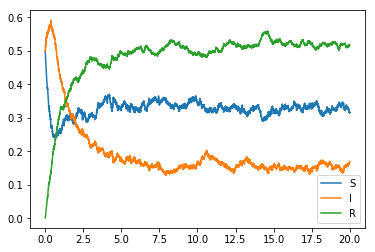
\includegraphics{figure1.png}


On obtiens bien un resultat qui parait coherent au premier coup
d'oeil. Pour vérifier cette simulation on résout l'equation
différentielle qui régit ce système:

\begin{eqnarray*}
  f'(x) &=& \sum_{x \in L}x\beta_x
\end{eqnarray*}

\begin{lstlisting}[frame=single]
  def print_simu(taux,liste_transition,X,N,time,fix=-1):
    data=simu_cmtc(taux,liste_transition,X,N,time,"",fix)
    K=len(X)
    for i in range(K):
        plot(data[0],data[1][:,i],label=str(i))
    def drift(x):
    return (sum([liste_transition[i]*taux(i,x)
for i in range(len(liste_transition))],0))
    
    t = linspace(0,time,1000)

    for i in range(K):
        x = odeint( lambda x,t : drift(x), X, t)
        plot(t,x,'--')
    legend()
    show()
  \end{lstlisting}

cette fonction nous permet donc de tracer sur la même courbe la
simulation et la solution théorique du système.
Avec les quelques lignes de code suivantes on obtient:

\begin{lstlisting}
  print_simu(taux,liste_transitions,X,1000,20)
\end{lstlisting}
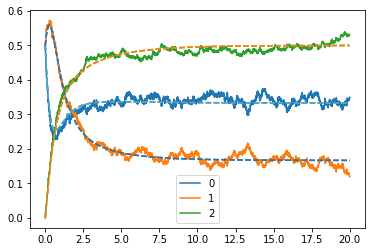
\includegraphics{figure2.png}

On a donc la confirmation que pour ce système la simulation est
coherente avec la résultet théorique. (l'ordre de grandeur et le signe
sont equivalnts).

\section{Calcule du coefficient en 1/N}

\subsection{Par simulation}

Pour calculer le coefficiet en 1/N on fait la moyenne des
points fixe obtenues lors de n simulation puis on soustrait a
ça le points fix calculé théoriquement: $C =
\frac{\sum_{i=0}^{n-1}{E(X^{(N)}_i)}}{n}-X_0 \ $

Pour calculer le point fixe par simulation on fait une moyenne sur le
dernier tier des termes d'une simulation longue (assez longue pour
qu'on ateigne largement le point fixe).

Mais le résultat de $C \ $ ne corespond pas! un autre terme d'erreur en
$O(\frac{1}{N}$ est aparue lors du calcul des points fixes par
simulation. La moyenne calculé des termes de la simulation ne prend
pas en compte le temps entre chaque transition d'où ce terme en
$O(\frac{1}{N})$.

Pour y remédier on calcule une moyenne pondéré par le temps entre
chaque transition.

\begin{lstlisting}[frame=single]
  def moy_pond(data,deb,fin,i):
    m=0
    for j in range(deb,fin):
        m+= data[1][j][i]*(data[0][j]-data[0][j-1])
    m=m/(data[0][fin-1]-data[0][deb-1])
    return(m)
\end{lstlisting}

on test donc de calculer ce coefficient sur un grand nombre de
simulations et pour des valeurs différentes de N. On est censsé
obtenir un résultat indépendant de N.
\newpage

\begin{lstlisting}[frame=single]
  N=linspace(10,1000,20)
  diff=array([[0. for i in N] for j in range(3)])
  C_i=array([[0. for i in N] for j in range(3)])
  X_0=fixed_point(taux,liste_transitions,3)

  for n in range(len(N)):
    for j in range(100):
      data=simu_cmtc(taux,liste_transitions,X,N[n],50)
        for i in range(3):
        diff[i,n]+=(moy_pond(data,int(len(data[1])/2),
                    len(data[1]),i)-X_0[i])/100.
    for i in range(3):
      C_i[i,n]=N[n]*diff[i,n]

  for i in range(3):
    plot(N,C_i[i,:])
  legend(('S','I','R'))
  show()
\end{lstlisting}

On obtient alors:

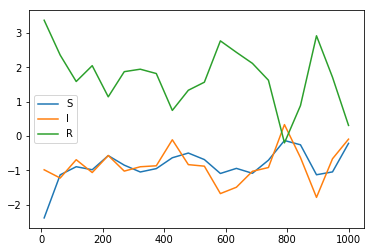
\includegraphics{figure3.png}

On observe un bruit important pour les grandes valeurs de N ce qui est
surrement du aux erreurs de calculs sur les réels avec python. On
observe donc $x_s=-1 \ x_I=-1\ x_R=2$ avec un bruit important pour 100
simulations par point. le temps de calcul pour ce résultat est
d'environ 40 minutes (avec un code non optimisé).

\subsection{Comparaison avec le calcul théoriquede ce coefficient}
On peut montrer que le coefficient d'erreur en $\frac{1}{N} \ $ vaut
exactement: \cite{meanfieldaprox}

\begin{eqnarray*}
  C_i=\frac{1}{2}*\sum_{j}((A^{-1})_{i,j}*\sum_{k_1,k_2}(B_j)_{k_1,k_2}W_{k_1,k_2})
\end{eqnarray*}

avec:
\begin{itemize}
\item $A_{i,j}=Df(x^*)_{i,j}$
\item $(B_j)_{k,l}=$
\item $W \ $ est la solution de l'équation de Lyapunov suivante: $AX+XA^T+Q=0$
\item Avec $Q=\sum_{l \in L} Q_l$
\item et $(Q_l)_{n,m}=-l_nl_m \beta_l(x^*)$
\end{itemize}

L'implémentation de ce calcule est réalisé a l'aide du module de
calcul symbolique de python: sympy.

\newpage
\begin{lstlisting}[frame=single]
  def theorique(taux,liste_transitions,n,dim):
    number_transitions = len(liste_transitions)  
    X_0 = fixed_point(taux,liste_transitions,n)
    
    Var=array([sym.symbols('x_{}'.format(i)) for i in range(n)])
    
    #print(len(X_0))
    f_x=array([0 for i in range(n)])
    for i in range(number_transitions):
        f_x = f_x + liste_transitions[i]*taux(i,Var)

    if dim==n-1:
        for i in range(n):
            f_x[i]=f_x[i].subs(Var[-1],1-sum(array([Var[i] 
                                                for i in range(n-1)])))

    A=array([[sym.lambdify(Var ,sym.diff(f_x[i],Var[j]))(*[X_0[k] 
                for k in range(n)]) 
              for j in range(dim)] 
             for i in range(dim)])

    B=array([[[sym.lambdify(Var,sym.diff(f_x[j],Var[k],Var[l]))(*[X_0[i] 
                for i in range(n)]) 
               for l in range(dim)] 
              for k in range(dim)] 
             for j in range(dim)])

    Q=array([[0. for i in range(dim)] for j in range(dim)])

    for l in range(number_transitions):
        Q += array([[liste_transitions[l][p]*liste_transitions[l][m]*taux(l,X_0) 
                     for m in range(dim)] 
                    for p in range(dim)])


    #print('A=',A)
    #print('Q=',Q)
    #print('B=',B)
    
    W = solve_lyapunov(A,Q)
    #print('W=',W)
    #print('sumW=',sum(W,0))

    A_inv=inv(A)
    
    C=[ 0.5*sum(array([A_inv[i][j]*sum(array([[B[j][k_1][k_2]*W[k_1][k_2] 
                                         for k_2 in range(dim)] 
                                        for k_1 in range(dim)])) 
                 for j in range(dim)])) 
       for i in range(dim)]
    for i in range(len(C)):
        C[i]=sum(C[i])
    return(C)
\end{lstlisting}

Cette fonction nous permet donc de calculer le coefficient de manière
théorique. Mais les systèmes étudiés ont souvent cette equation de
vérifié:
\begin{eqnarray*}
  \sum_{x \in X}x &=& 1
\end{eqnarray*}
le système SIR par exemple vérifie $x_S+x_I+x_R=1$. donc on étudie n
système de dimention 2 et non 3. Il faut donc le préciser a l'entrée
de la fonction: $n=3 \ et \ dim=2$.

\begin{lstlisting}[frame=single]
  theorique(taux,liste_transitions,3,2)
\end{lstlisting}

On obtient: $[-0.75000000000000111,\ -0.96428571428571352]$
Ce qui corespond bien aux valeurs calculés par simulation. Ce calcul
n'a pris que quelques secondes a calculer comparé aux 40 minutes du
résultat approximatif des simulations.

Pour un exemple simple comme le système SIR on a déjà des problèmes de
temps de calcul par simulation. La formule précedente facilite donc
grandement le calcul du coefficient en 1/N.


\section{Exemples étudiés}

\subsection{Bianchi's formula}
On s'interesse ici a un modèle \cite{bianchi} pour le protocole 802.11 MAC. On le
modelise a l'aide d'une chaine de markov. On obtient la chaine de
markov aux transitions suivantes:

\begin{eqnarray*}
  x & \rightarrow & x+e_0-e_k \ avec\ un\ taux \
  q_kx_k\prod_{m=0}^K(1-\frac{q_m}{N})^{Nx_m-e_k} \ for \ k \in
                    \{1...K-1\} \\
  x & \rightarrow & x+e_{k+1}-e_k \ avec\ un\ taux \
  q_kx_k(1-\prod_{m=0}^K(1-\frac{q_m}{N})^{Nx_m-e_k}) \ for \ k \in
                    \{1...K-1\} \\
  x & \rightarrow & x+e_0-e_K \ avec \ un \ taux \ q_Kx_K
\end{eqnarray*}

On entre alors le système de la manière suivante dans notre
simulateur:

\newpage
\begin{lstlisting}[frame=single]
N=100
K=5
Var_x=array([sym.symbols('x_{}'.format(i)) for i in range(K)])
#Var_q=array([sym.symbols('q_{}'.format(i)) for i in range(K)])
Var_q=array([2**(-i) for i in range(K)])

def mult_liste(Liste):
    S=1
    for i in Liste:
        S*=i
    return(S)

E=[array([1 if i==j else 0 for j in range(K)]) for i in range(K)]

liste_transitions =[]
taux=[]

liste_transitions.append(E[1]-E[0])
taux.append(Var_q[0]*Var_x[0]*
(1-mult_liste([(1-Var_q[m]/N)**(N*Var_x[m]-(0 if m!=0 else 1)) 
                                            for m in range(K)])))

for i in range(1,K-1):
    liste_transitions.append(E[0]-E[i])
    taux.append(Var_q[i]*Var_x[i]*
    mult_liste([(1-Var_q[m]/N)**(N*Var_x[m]-(0 if m!=i else 1)) 
                                              for m in range(K)]))
    liste_transitions.append(E[i+1]-E[i])
    taux.append(Var_q[i]*Var_x[i]*
    (1-mult_liste([(1-Var_q[m]/N)**(N*Var_x[m]-(0 if m!=i else 1)) 
                                                 for m in range(K)])))

liste_transitions.append(E[0]-E[K-1])
taux.append(Var_q[K-1]*Var_x[K-1])

def fct_taux(i,X):
    return sym.lambdify( Var_x,taux[i])(*X)
\end{lstlisting}

Puis on entre les conditions initiales et on trace le tout:

\begin{lstlisting}[frame=single]
X=[1/K for i in range(K)]
print_simu(fct_taux,liste_transitions,X,1000,15)
\end{lstlisting}

On obtient la figure suivante:

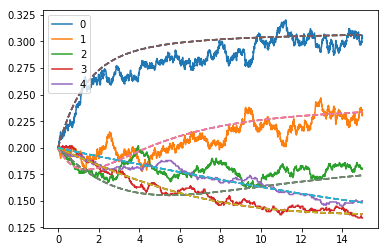
\includegraphics{bianchi.png}

\subsection{Velo'v}
La répartition et l'évolution du nombre de vélo par stations de velo'v
peut facilement se traduire en une chaine de markov. On peut utiliser
un tel modèle \cite{velov} pour optimiser le nombre de velo par station par
exemple.

\begin{lstlisting}[frame=single]
K=10
N=20
s=3
Lambda=1
Mu=0.5

y=array([sym.symbols('y_{}'.format(i)) for i in range(K)])
E=[array([1 if i==j else 0 for j in range(K)]) for i in range(K)]
liste_transition=[]
taux=[]

for i in range(K-1):
    liste_transition.append(E[i+1]-E[i])
    taux.append(Mu*y[i]*(s-sum([n*y[n] for n in range(K)])))
    
for i in range(1,K):
    liste_transition.append(E[i-1]-E[i])
    taux.append(Lambda*y[i])
    
def fct_taux(i,X):
    return(sym.lambdify(y,taux[i])(*X))
\end{lstlisting}

Il nous reste plus qu'a choisir une distribution initiale et a tracer
l'évolution.

\begin{lstlisting}[frame=single]
X=[1,0,0,0,0,0,0,0,0,0]
print_simu(fct_taux,liste_transition,X,100,10)
\end{lstlisting}

On obtient alors la courbe suivante:

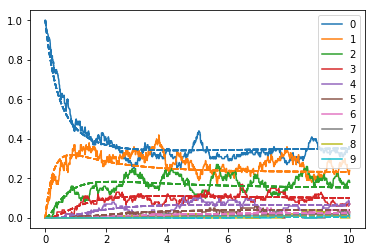
\includegraphics{velov.png}

\section{Librairie contenant l'ensemble du code}
L'ensemble du code est rassemblé dans une librairie python3
\cite{librairie} qui
contient les fonctions suivantes:
\begin{itemize}
  \item
    $simu\_ctmc(fct\_taux,liste\_transition,X_0,N,temps\_final,'mon\_fichier.out',fix\_seed)
    \ $
    qui simule notre CMTC.
  \item $file\_to\_array('mon\_fichier.out',len(X)) \ $ qui permet de
    récuperer les données si on les a stockés dans un fichier
    précedement.
  \item $fixed\_point(taux,liste\_transition,n) \ $ qui renvoit un vecteur
    des points fixes du système calculés a l'aide de odeint.
  \item $theorique(taux,liste_transition,n,dim)$ qui calcule le
    coeficient d'erreur $C \ $ de manière théorique.
\end{itemize}

\bibliographystyle{plain}
\bibliography{bibli}

\end{document}
